Software architecture is complex, and require a lot of details. In order to  describe the entire architecture of the software made in this project, separating the architecture into different views is a necessity. An architectural view is a description of the architecture as seen from different stakeholders. 

 One view model to use is the 4+1 View Model, which contains the four views: logical, development, process and physical view. An additional view is the scenario view, which is redundant with the other views, but provide an overview over the needed components in the other views. The scenarios describe the system through the use of use cases, and is basically an abstraction of the most important requirements specified in the functional requirements.  The architectural drivers described in section \ref{drivers} are based on the scenario view.
 
 The architecture in this project will mainly be based off the logical and development views. The logical view is concerned with the functionality the system delivers to the end-user. The reason for choosing the logical view is pretty obvious; the end-user is the main stakeholder for the project, and providing the required functionality determines the success of the product. 
 
 \subsection{Logical View}

There are two approaches on how to represent the logical view, object oriented or data driven. Since this project will be programmed in Java, and after considering how Java abstracts data into objects, the object oriented approach was chosen. The logical view is then represented through the use of class diagrams and class templates.  Internal behavior of an object is described with state transition diagrams or state charts. State transition diagram will be made in later stages of the project, when a more detailed picture of the functionality can be made. \cite{4plus1view}

\begin{figure}[h]
	\center
	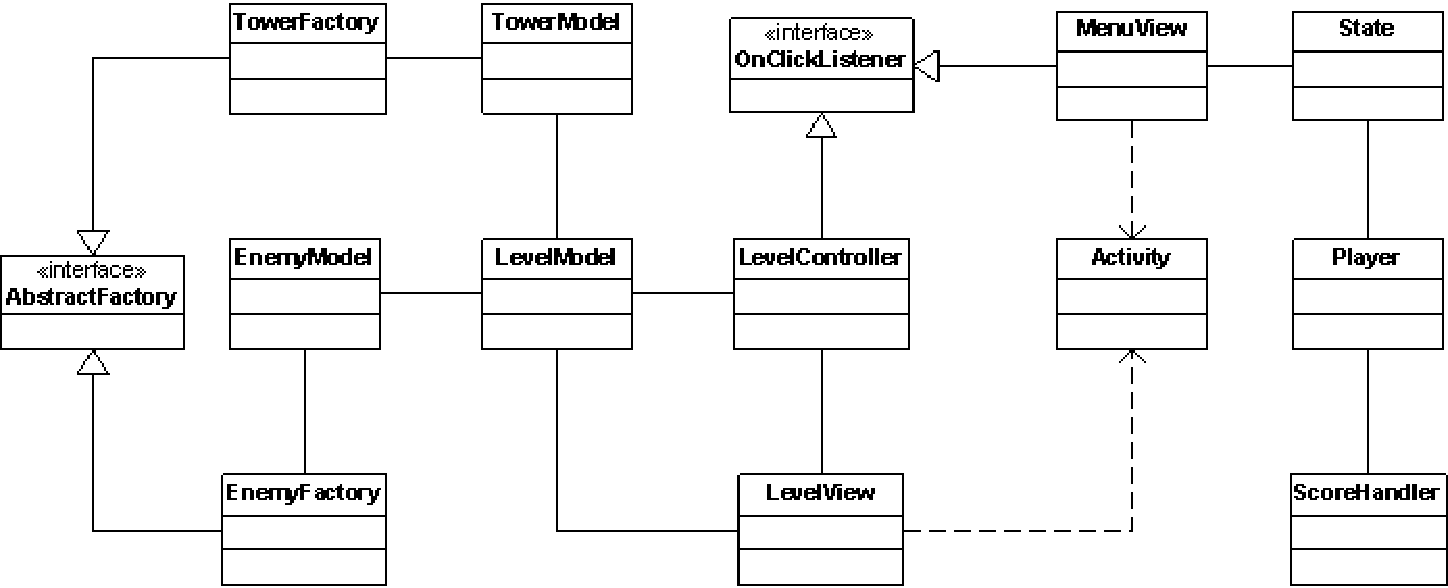
\includegraphics[width=1\linewidth ]{images/class_diagram.png}
%	\label{fig:class_diagram}
	\caption{Class diagram for the logical view}
\end{figure}
\subsection{Development View}

 The development view describe the system from a programmers viewpoint, mainly through the use of UML Component diagram or a UML package diagram which we will use.  The development view is for example concerned with partitioning, grouping and visibility. The quality attributes for this project, as specified in in the requirements document \cite{reqdoc} are maintainability and testability. These are attributes which are described in the development view, thus including the development view is a necessity. 


Below is a package diagram showing the preliminary development view of our tower defense game. The diagram is showing the various packages and classes within. As the diagram shows, some of the package names illustrate the use of the MVC-pattern, and the association between the different modules.

\begin{figure}[h]
\center
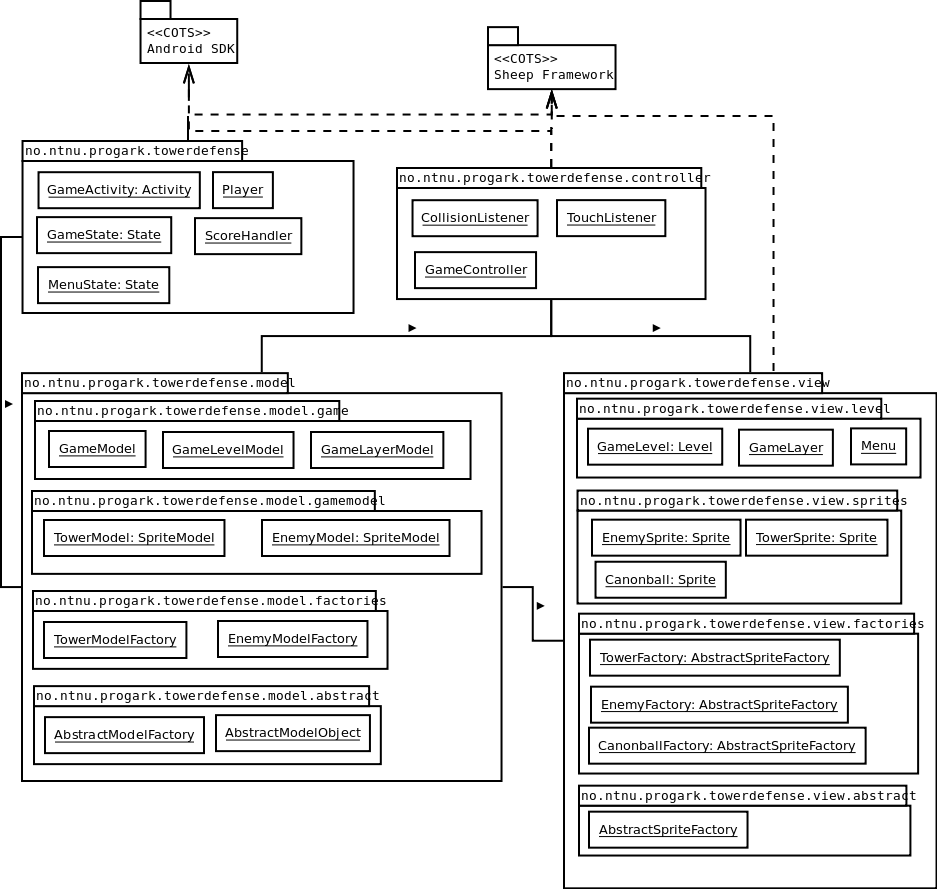
\includegraphics[width=1\linewidth ]{images/pDiagram.png}
%\label{fig:package_diagram}
\caption{Package diagram}
\end{figure}

The model package includes the various models needed to manage the underlying functionality of all the active sprites in the game as well as the actual gamestate. 


The controller package includes the action- and eventlisteners such as the CollisionListener, which will be invoked if two sprites collide in-game. There is also a GameController which includes controllers related to the gamestate, such as the LevelController. This class should probably be divided into more classes, depending on how big responsibility it receives. Regarding the responsibility delegation it should be worth mentioning that we try to keep in mind the Single-responsibility principle, in which a class should have only one responsibility. If it has more than one, we separate it into more classes.

The view package includes Sprite-classes and other elements which will be drawn on the screen. These classes should only contain functionality for drawing and animating stuff on the screen.

The COTS libraries, Android SDK and the Sheep framework, are also illustrated in the diagram, showing the dependencies drawn from these.
